\documentclass[unicode,12pt,a4paper,oneside,numbers=endperiod,openany]{scrartcl}
\setlength{\parindent}{0em}

\usepackage{ifthen}
\usepackage[utf8]{inputenc}
\usepackage{graphics}
\usepackage{graphicx}
\usepackage{hyperref}

\usepackage[T1]{fontenc}
\usepackage{helvet}
\usepackage{etoolbox}

\usepackage{xcolor}
\usepackage{listings}
\definecolor{vgreen}{RGB}{104,180,104}
\definecolor{vblue}{RGB}{49,49,255}
\definecolor{vorange}{RGB}{255,143,102}

\lstdefinestyle{verilog-style}
{
    language=Verilog,
    basicstyle=\small\ttfamily,
    keywordstyle=\color{vblue},
    identifierstyle=\color{black},
    commentstyle=\color{vgreen},
    numbers=left,
    numberstyle=\tiny\color{black},
    numbersep=10pt,
    tabsize=8,
    moredelim=*[s][\colorIndex]{[}{]},
    literate=*{:}{:}1
}

\makeatletter
\newcommand*\@lbracket{[}
\newcommand*\@rbracket{]}
\newcommand*\@colon{:}
\newcommand*\colorIndex{%
    \edef\@temp{\the\lst@token}%
    \ifx\@temp\@lbracket \color{black}%
    \else\ifx\@temp\@rbracket \color{black}%
    \else\ifx\@temp\@colon \color{black}%
    \else \color{vorange}%
    \fi\fi\fi
}
\makeatother
\pagestyle{plain}
\voffset -5mm
\oddsidemargin  0mm
\evensidemargin -11mm
\marginparwidth 2cm
\marginparsep 0pt
\topmargin 0mm
\headheight 0pt
\headsep 0pt
\topskip 0pt        
\textheight 255mm
\textwidth 165mm

\newcommand{\duedate} {}
\newcommand{\setduedate}[1]{%
\renewcommand\duedate {Due date:~ #1}}
\newcommand\isassignment {false}
\newcommand{\setassignment}{\renewcommand\isassignment {true}}
\newcommand{\ifassignment}[1]{\ifthenelse{\boolean{\isassignment}}{#1}{}}
\newcommand{\ifnotassignment}[1]{\ifthenelse{\boolean{\isassignment}}{}{#1}}

\newcommand{\assignmentpolicy}{
\begin{table}[h]
\begin{center}
\scalebox{0.8} {%
\begin{tabular}{|p{0.02cm}p{16cm}|}
\hline
&\\
\multicolumn{2}{|c|}{\Large\textbf{HPC  2021 ---  Submission Instructions}}\\
\multicolumn{2}{|c|}{\large\textbf{(Please, notice that following instructions are mandatory: }}\\
\multicolumn{2}{|c|}{\large\textbf{submissions that don't comply with, won't be considered)}}\\
&\\
\textbullet & Assignments must be submitted to \href{https://www.icorsi.ch/course/view.php?id=12615}{iCorsi} (i.e. in electronic format).\\
\textbullet & Provide both executable package and sources (e.g. C/C++ files, Matlab). 
If you are using libraries, please add them in the file. Sources must be organized in directories called:\\
\multicolumn{2}{|c|}{\textit{Project\_number\_lastname\_firstname}}\\
& and  the  file must be called:\\
\multicolumn{2}{|c|}{\textit{project\_number\_lastname\_firstname.zip}}\\
\multicolumn{2}{|c|}{\textit{project\_number\_lastname\_firstname.pdf}}\\
\textbullet &  The TAs will grade your project by reviewing your project write-up, and looking at the implementation 
                 you attempted, and benchmarking your code's performance.\\

\textbullet & You are allowed to discuss all questions with anyone you like; however: (i) your submission must list anyone you discussed problems with and (ii) you must write up your submission independently.\\
\hline
\end{tabular}
}
\end{center}
\end{table}
}
\newcommand{\punkte}[1]{\hspace{1ex}\emph{\mdseries\hfill(#1~\ifcase#1{Points}\or{Points}\else{Points}\fi)}}


\newcommand\serieheader[6]{
\thispagestyle{empty}%
\begin{flushleft}

\includegraphics[width=0.3\textwidth]{usi_inf.png}
\end{flushleft}
  \noindent%
  {\large\ignorespaces{\textbf{#1}}\hspace{\fill}\ignorespaces{ \textbf{#2}}}\\ \\%
  {\large\ignorespaces #3 \hspace{\fill}\ignorespaces #4}\\
  \noindent%
  \bigskip
  \hrule\par\bigskip\noindent%
  \bigskip {\ignorespaces {\Large{\textbf{#5}}}
  \hspace{\fill}\ignorespaces \large \ifthenelse{\boolean{\isassignment}}{\duedate}{#6}}
  \hrule\par\bigskip\noindent%  \linebreak
 }

\makeatletter
\def\enumerateMod{\ifnum \@enumdepth >3 \@toodeep\else
      \advance\@enumdepth \@ne
      \edef\@enumctr{enum\romannumeral\the\@enumdepth}\list
      {\csname label\@enumctr\endcsname}{\usecounter
        {\@enumctr}%%%? the following differs from "enumerate"
	\topsep0pt%
	\partopsep0pt%
	\itemsep0pt%
	\def\makelabel##1{\hss\llap{##1}}}\fi}
\let\endenumerateMod =\endlist
\makeatother




\usepackage{textcomp}


\lstdefinestyle{mystyle}{
    language=C,                     % the language of the code
    basicstyle=\ttfamily\small,      % the size of the fonts that are used for the code
    keywordstyle=\color{blue},       % keyword style
    stringstyle=\color{red},         % string literal style
    commentstyle=\color{magenta},      % comment style
    morecomment=[l][\color{magenta}]{\#}
}




\usepackage{float}	
\usepackage{caption}	
\usepackage{pdflscape}
\usepackage{multirow}
\usepackage{enumitem}
\setitemize{noitemsep,topsep=6pt,parsep=6pt,partopsep=6pt}
\usepackage[font=itshape]{quoting}

\lstset{basicstyle=\footnotesize\ttfamily,breaklines=true}
\lstset{framextopmargin=5pt,framexbottommargin=5pt}
\lstset{literate=
    {─}{{\pmboxdrawuni{2500}}}1 
    {├}{{\pmboxdrawuni{251C}}}1 
    {└}{{\pmboxdrawuni{2514}}}1
	{│}{{\pmboxdrawuni{2502}}}1
}
\lstset{aboveskip=10pt,belowskip=10pt,captionpos=b,abovecaptionskip=6pt}

\begin{document}

\setassignment
\setduedate{21.12.2023}

\serieheader{Edge Computing in the IoT | Group Project Report}{Fall 2023}{Authors: Alfio Vavassori, Cristiano Colangelo, Edoardo Riggio, Samuel Corecco}{}{\large{IoT Solar Station}}{}

\tableofcontents

\newpage

\section{Abstract}

The IoT Solar Station is an advanced weather station with an integrated
self-positioning solar panel. The orthogonal 2-axis servo motors move the solar
panel, while the attached voltmeter constantly measures the current power
production. The solar panel moves at different angles and searches for the best
one based on the voltmeter measurements. The onboard sensors send the collected
data to a private MQTT broker, which forwards the data to a Python backend. The
backend ingests the data into a DigitalOcean cloud instance hosting an
ElasticSearch database via Docker containers. Finally, a Kibana dashboard
deployed alongside the database showcases the collected data in nice, compact
visualizations. 

\section{Hardware}
Regarding the hardware used in this project, Figure~\ref{fig:circuit} shows a complete overview of which elements have been used and how they were connected.
\begin{figure}[h]
    \centering
    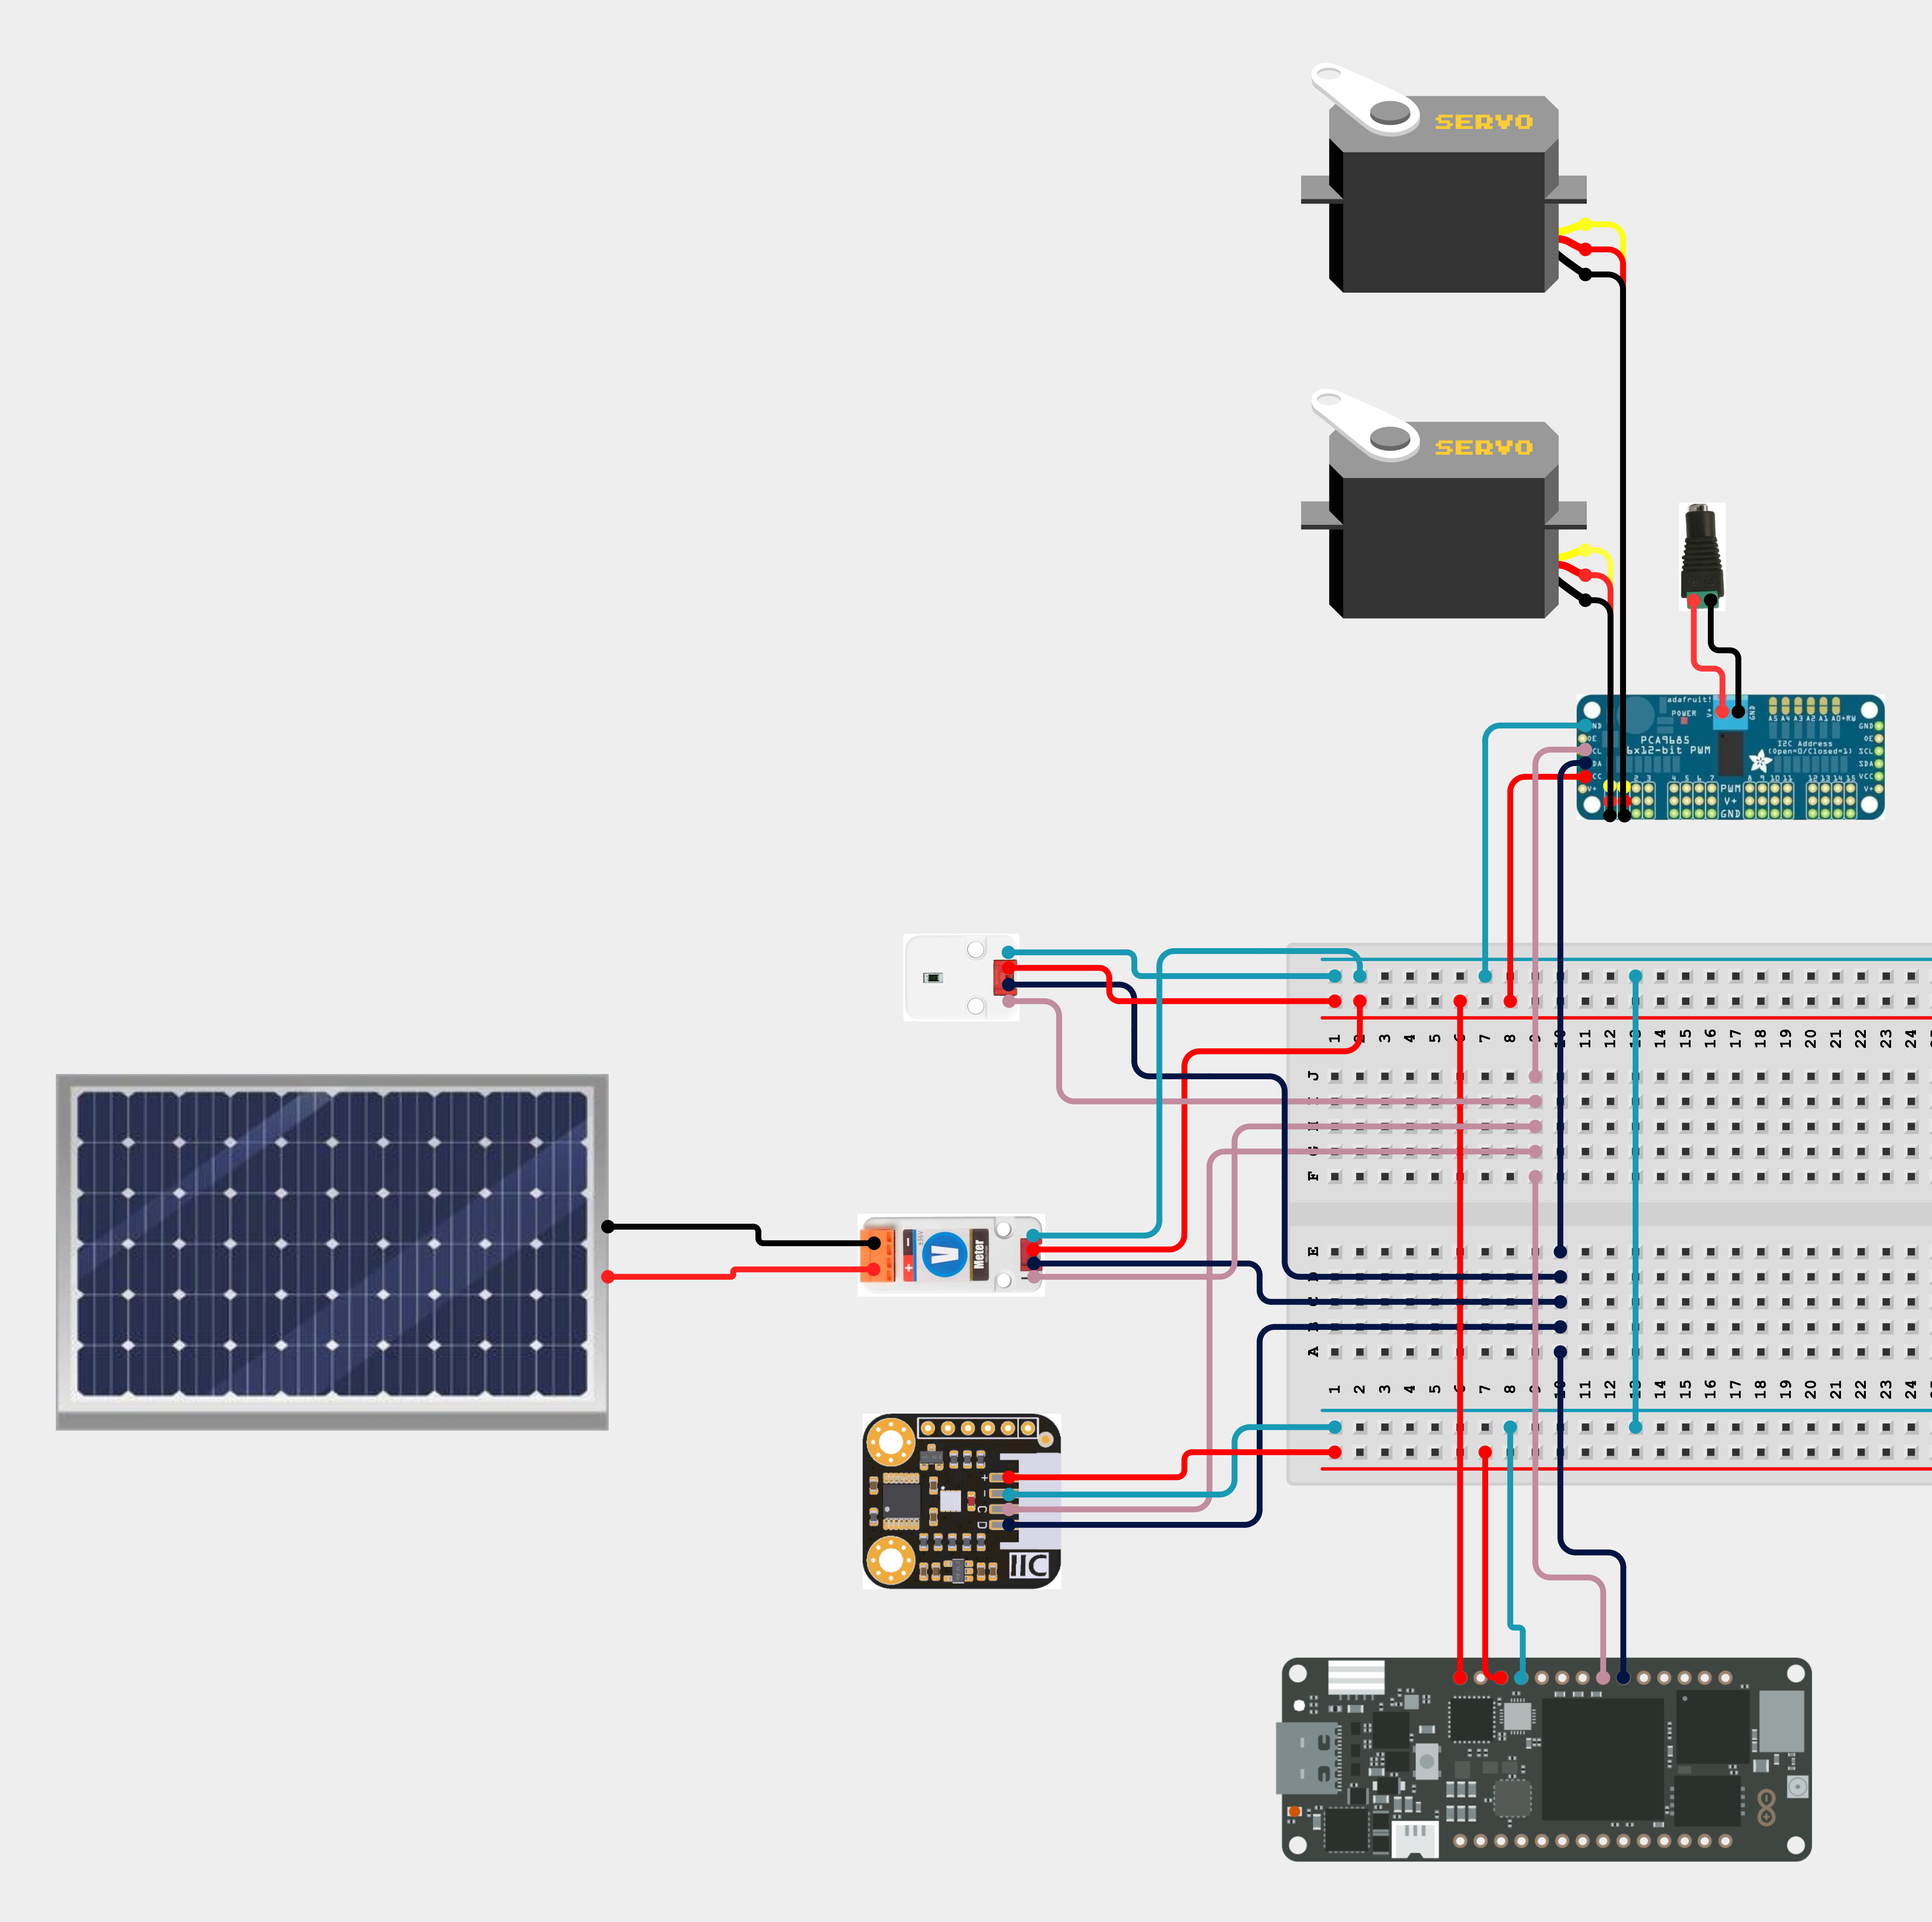
\includegraphics[width=10cm]{../assets/png/project-circuit}
    \caption{Overview of the hardware used in our project.}
    \label{fig:circuit}
\end{figure}
The parts used where: two servos, a motor shield, a light intensity sensor, a
voltmeter connected to a solar panel, an ambient sensor, and an Arduino Portenta
H7. All the components were connected to the Portenta board using the I2C
protocol. Please note that our delivered code, available in
\texttt{src/arduino/arduino.ino}, has been well commented and cleaned up. Setup
and loop code is well separated in the two homonoymous methods.

\subsection*{Servos}
The two servos are the responsible for the movement of the solar panel. These
are high-torque servos and are attached to a 3D-printed structure that holds the
solar panel and moves it on two different planes. The bottom servo rotates the
panel, while the top servo adjusts the inclination of the panel. \\ \\
To be able to interface with the Arduino board, we used a motor shield to which we connected both servos.
Since they require some energy, the shield was connected to the wall outlet by means of a power supply cable. \\ \\
As part of the telemetry data, we also added a small piece of code that keeps
track of the orientation (NW = nord west, SO = south ovest, etc.). The IoT Solar
Station should be positioned initially toward the north direction, since it is a
closed-loop control algorithm for simplicity.

\begin{lstlisting}[style=mystyle,language=C,caption={The \texttt{get\_direction} function keeps track of the 2 rotation axis and computes the direction.}]
String get_direction(int servo_0, int servo_1) {
    String direction = "N";

    float tolerance = 115;
    float inclinations[3] = {300, 580, 640};
    float directions[4] = {150, 265, 380, 495};

    if (servo_0 >= directions[0] - tolerance && servo_0 <= directions[0] + tolerance) {
        direction = "N";
    } else if (servo_0 > directions[1] - tolerance && servo_0 <= directions[1] + tolerance) {
        direction = "NW";
    } else if (servo_0 > directions[2] - tolerance && servo_0 <= directions[2] + tolerance) {
        direction = "W";
    } else if (servo_0 > directions[3] - tolerance && servo_0 <= directions[3] + tolerance) {
        direction = "SW";
    }

    if (direction == "N" && servo_1 > inclinations[1]) {
        direction = "S";
    } else if (direction == "NW" && servo_1 > inclinations[1]) {
        direction = "SE";
    } else if (direction == "W" && servo_1 > inclinations[1]) {
        direction = "E";
    } else if (direction == "SW" && servo_1 > inclinations[1]) {
        direction = "NE";
    }

    return direction;
}
\end{lstlisting}

\subsection*{Ambient Sensor}
Attached to the system, there is an ambient sensor which will capture several
different measurements. These measurements are temperature, pressure, humidity,
and light intensity. These measurements are not used to drive the
best-position-seeking algorithm for the solar panel, but are used to populate
the weather station's dashboard.

\subsection*{Light Intensity Sensor}
As with the ambient sensor, the light intensity sensor does not serve a real
purpose towards the computation of the best position. The data taken from this
sensor is used in the weather station dashboard.

\subsection*{Voltmeter}

The system must actively adjust the solar panel in response to the position of
the sun, adjusting its position to maximize energy absorption. This is done with
two main actions, searching for the optimal position and scanning the various
positions and angles. \\ \\
Our model must also take into account times of low solar intensity such as
cloudy conditions or night. In these scenarios, our system enters an
energy-saving phase. The system will only capture sensor data, and as long as
the produced voltage does not exceed 1V, the system will not search for new
positions (Figure~\ref{fig:seros-sm}).
\begin{figure}[h]
    \centering
    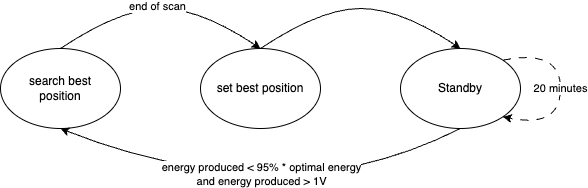
\includegraphics[width=12cm]{../assets/png/servos-state-machine}
    \caption{State machine that describes the lifecycle of our system.}
    \label{fig:seros-sm}
\end{figure}


\section{Communication}
\section*{Communication}

For our project, we decided to implement communication with an MQTT (MQ Telemetry Transport) broker, which allows us to send lightweight, continuous messages to our cloud instance.
We used the service shiftr.io, a high-performance broker that easily connects devices to the same network (Figure~\ref{fig:shiftrviz}). \\ \\
To implement communication, we used a MQTT client library in both the Arduino Portenta and our Python backend.
The MQTT client on the Arduino board will send a message after every calibration phase.
The client emits a JSON message on a defined topic, and the Python backend will subscribe to that topic.
When a message is sent from the Arduino, the Python server will receive the message which will then be sent to our ElasticSearch.
\begin{figure}[H]
    \centering
    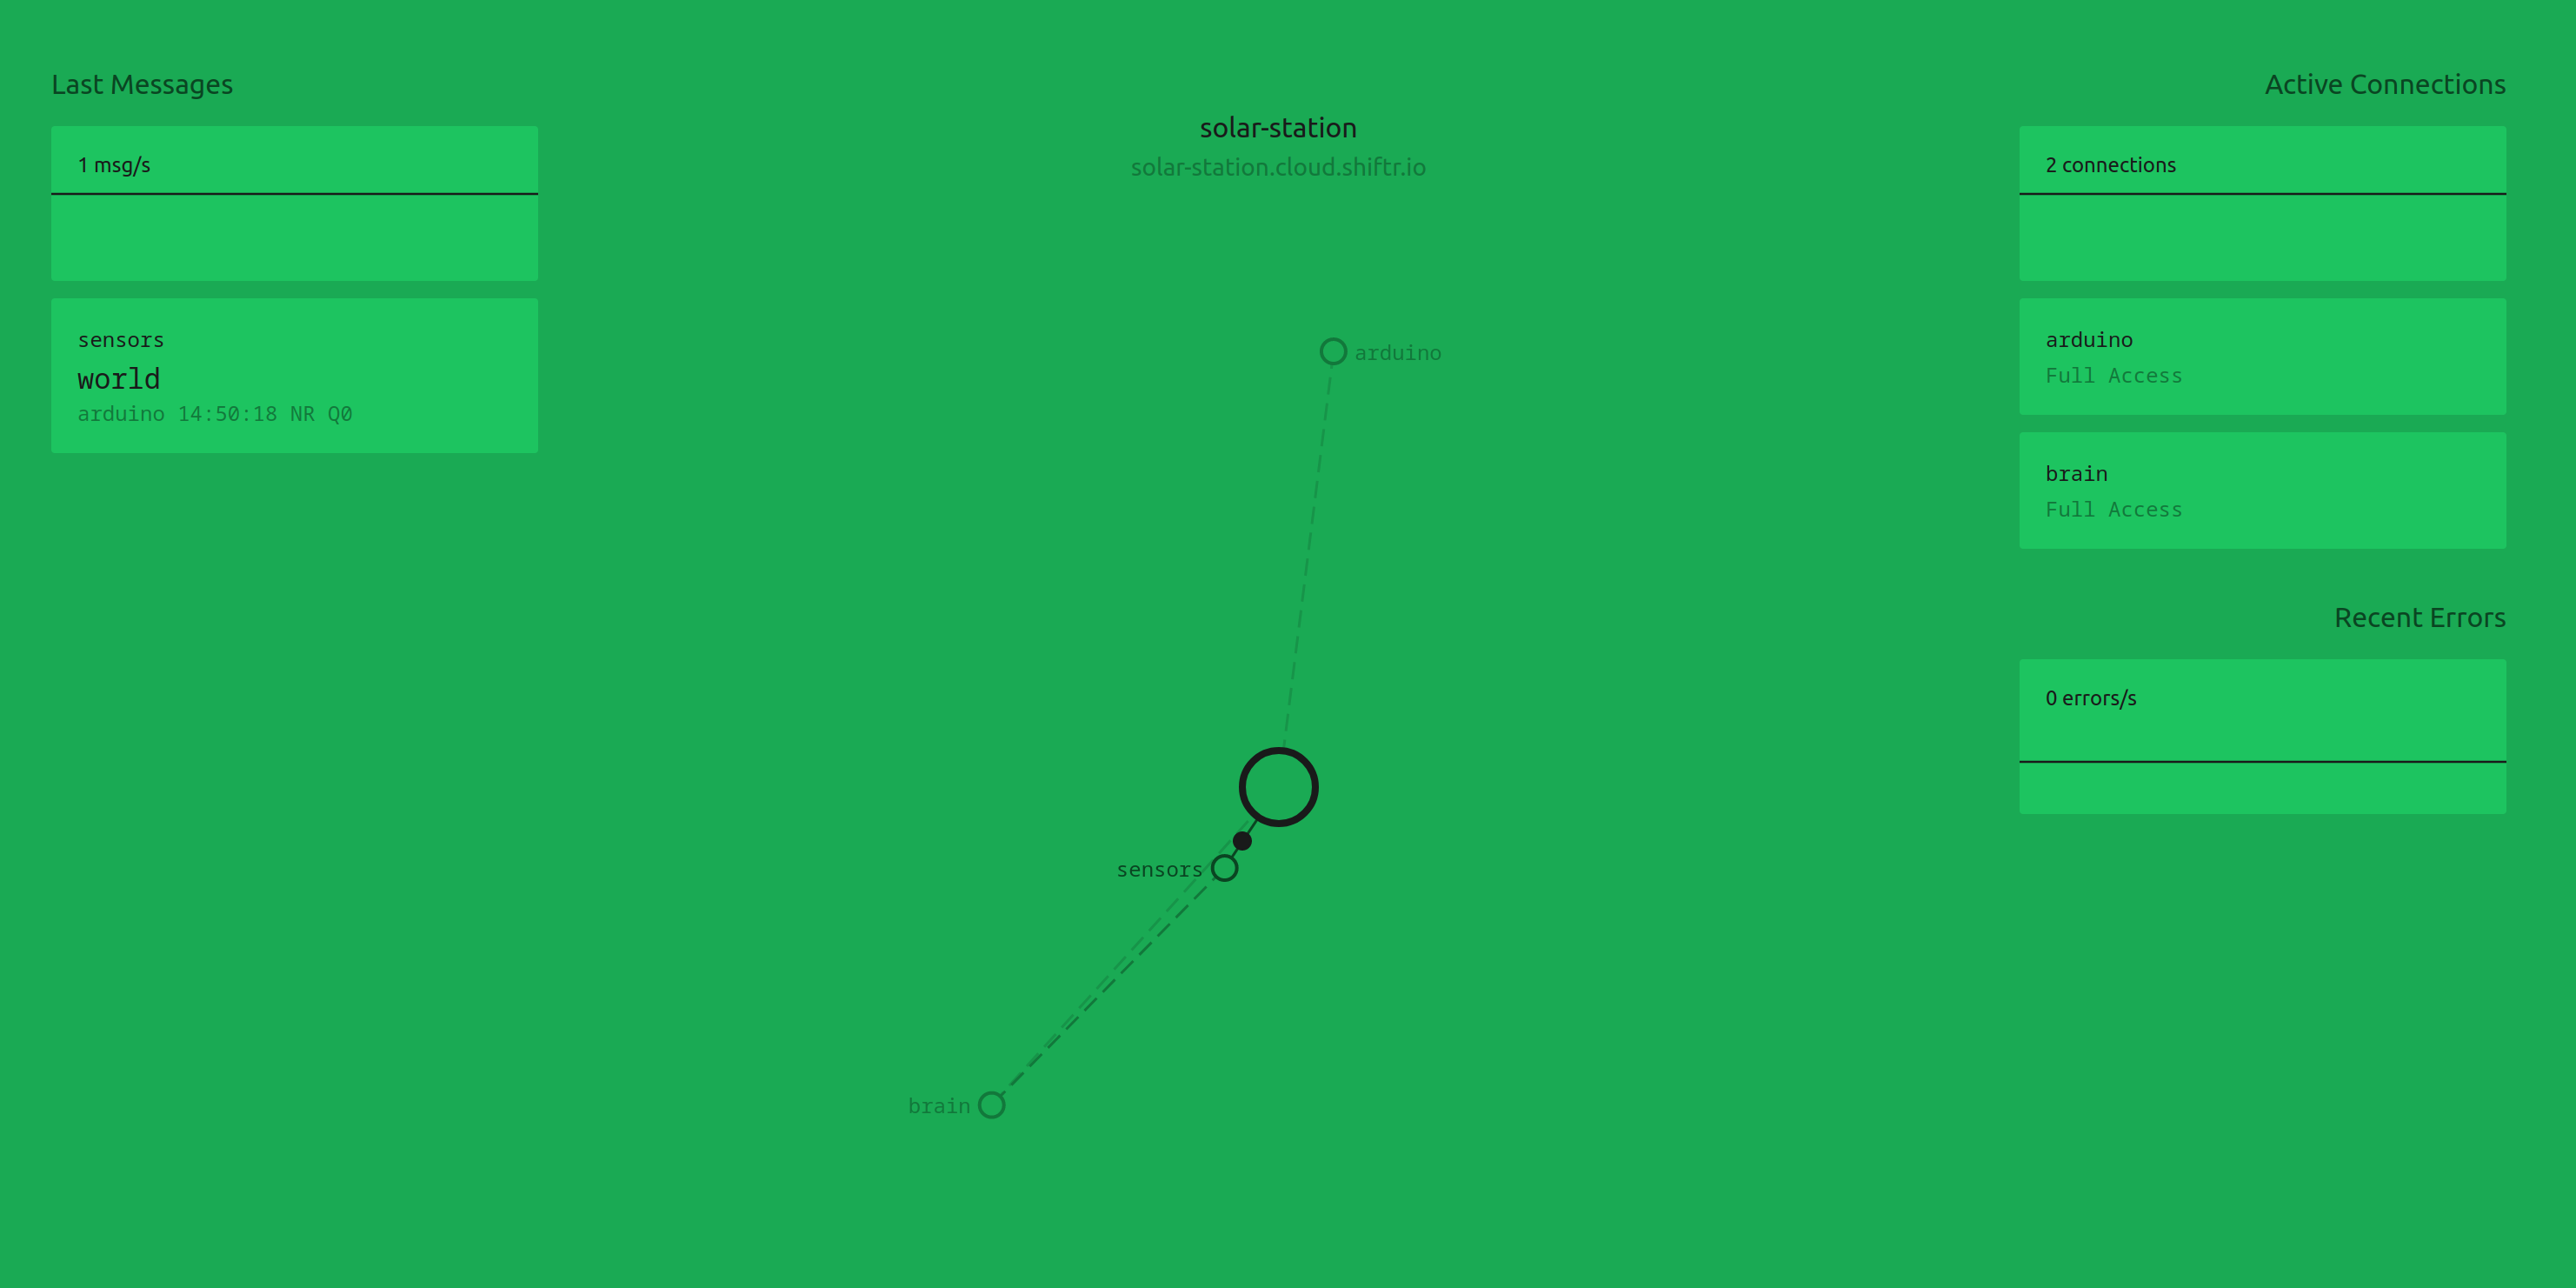
\includegraphics[width=15cm]{../assets/png/shiftr-network}
    \caption{Visualization of our MQTT network through the shiftr.io interface. The "arduino" dot represents our Arduino Portenta device, the "brain" dot represents our Python backend, and the "sensors" dot represents the topic where messages are published.}
    \label{fig:shiftrviz}
\end{figure}
In brief, we used the Arduino WiFi library to connect to the Internet.
We had troubles with USI's WiFi network, as it was necessary to authenticate, so we simply used our mobile hotspots.
We used the Python library Eclipse Paho \cite{paho} to make our Python client subscribe to the topic, which was trivial.
The respective library on the Arduino side is Arduino MQTT by Joël Gähwiler and contributors \cite{arduinomqtt}.


\section{3D structure}
\section*{Cloud setup}

For our cloud setup, we used Docker \cite{docker} containers running in a DigitalOcean \cite{do} instance (Figure~\ref{fig:do}).
We decided to install ElasticSearch \cite{es}, a RESTful search and analytics database that works well with its dashboard builder, Kibana \cite{kibana}.
The setup was relatively straightforward, but we had some troubles at first because we discovered ElasticSearch is a quite memory-intensive program, therefore we had to resize our cloud instance to have more RAM available, as well as research how to allocate more memory for Docker containers. \\ \\
\begin{figure}[H]
    \centering
    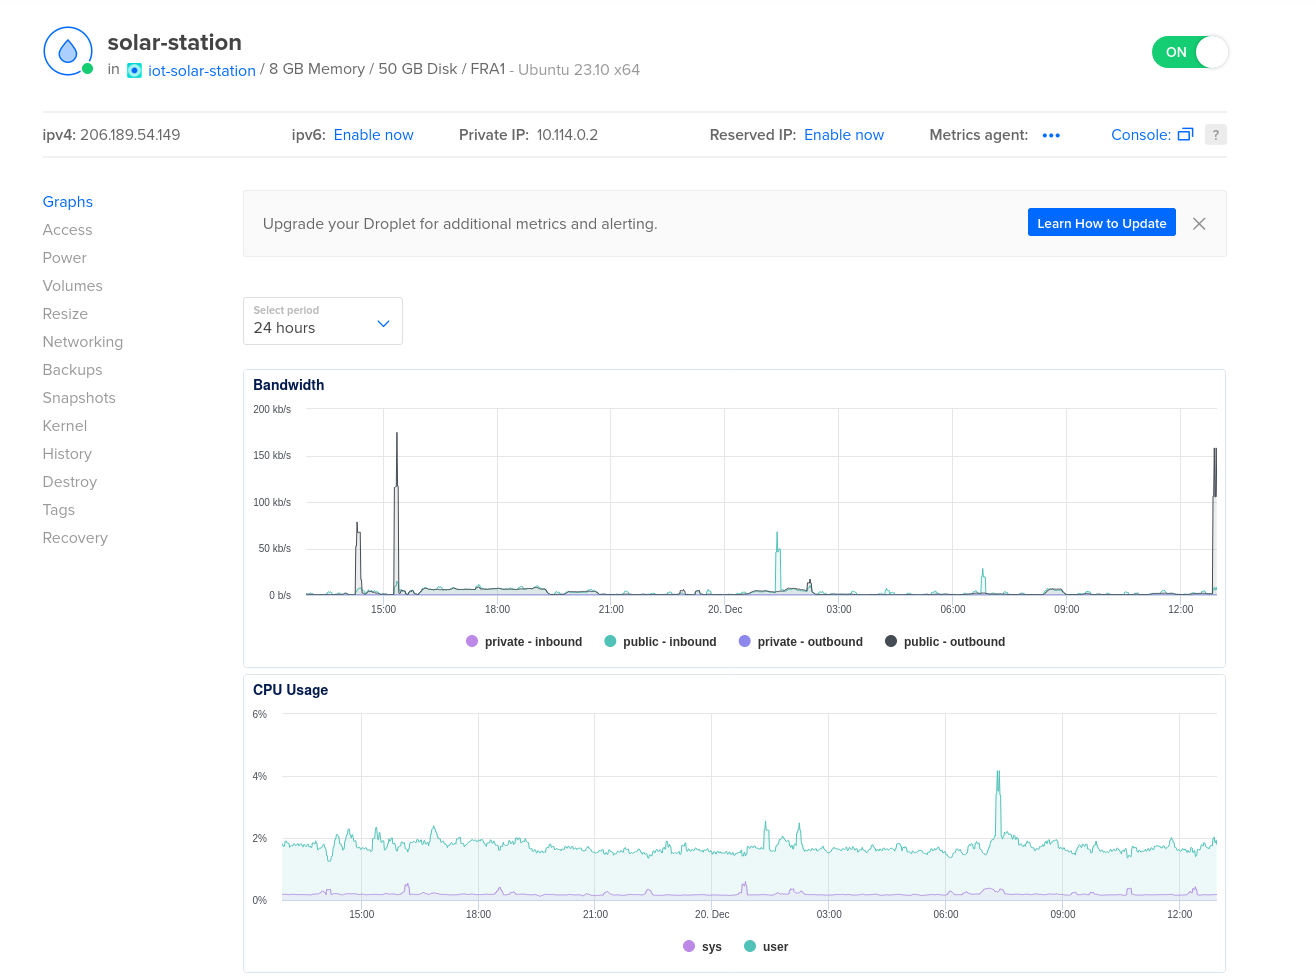
\includegraphics[width=\textwidth]{../assets/png/digital-ocean-graph}
    \caption{A sneak peek of the DigitalOcean interface showing some telemetry about our cloud instance.}
    \label{fig:do}
\end{figure}\
This allowed us to develop faster in the end because we had a shared database for measurement.
We could collaborate more easily asynchronously as we had the same development environment for everyone.
It is also a more realistic setup, although no HTTPS certificate was installed.
We also had to specify the necessary port-forwarding rules in the intuitive DigitalOcean web interface to allow outside connection. \\ \\
A list of the steps undertaken for this part can be found in file \texttt{scripts/es\_setup.sh} in the delivered zip.


\section{Dashboard}
To nicely visualize all the data we collected through the MQTT broker, we
decided to build a Kibana dashboard since it integrates seamlessly with our
ElasticSearch installation and provides a wide range of visualizations. We
visualize all the data we gather and plot them in linecharts and gauges with
unit of measurement as well. Please see the below screenshot.

\begin{figure}[H]
    \centering
    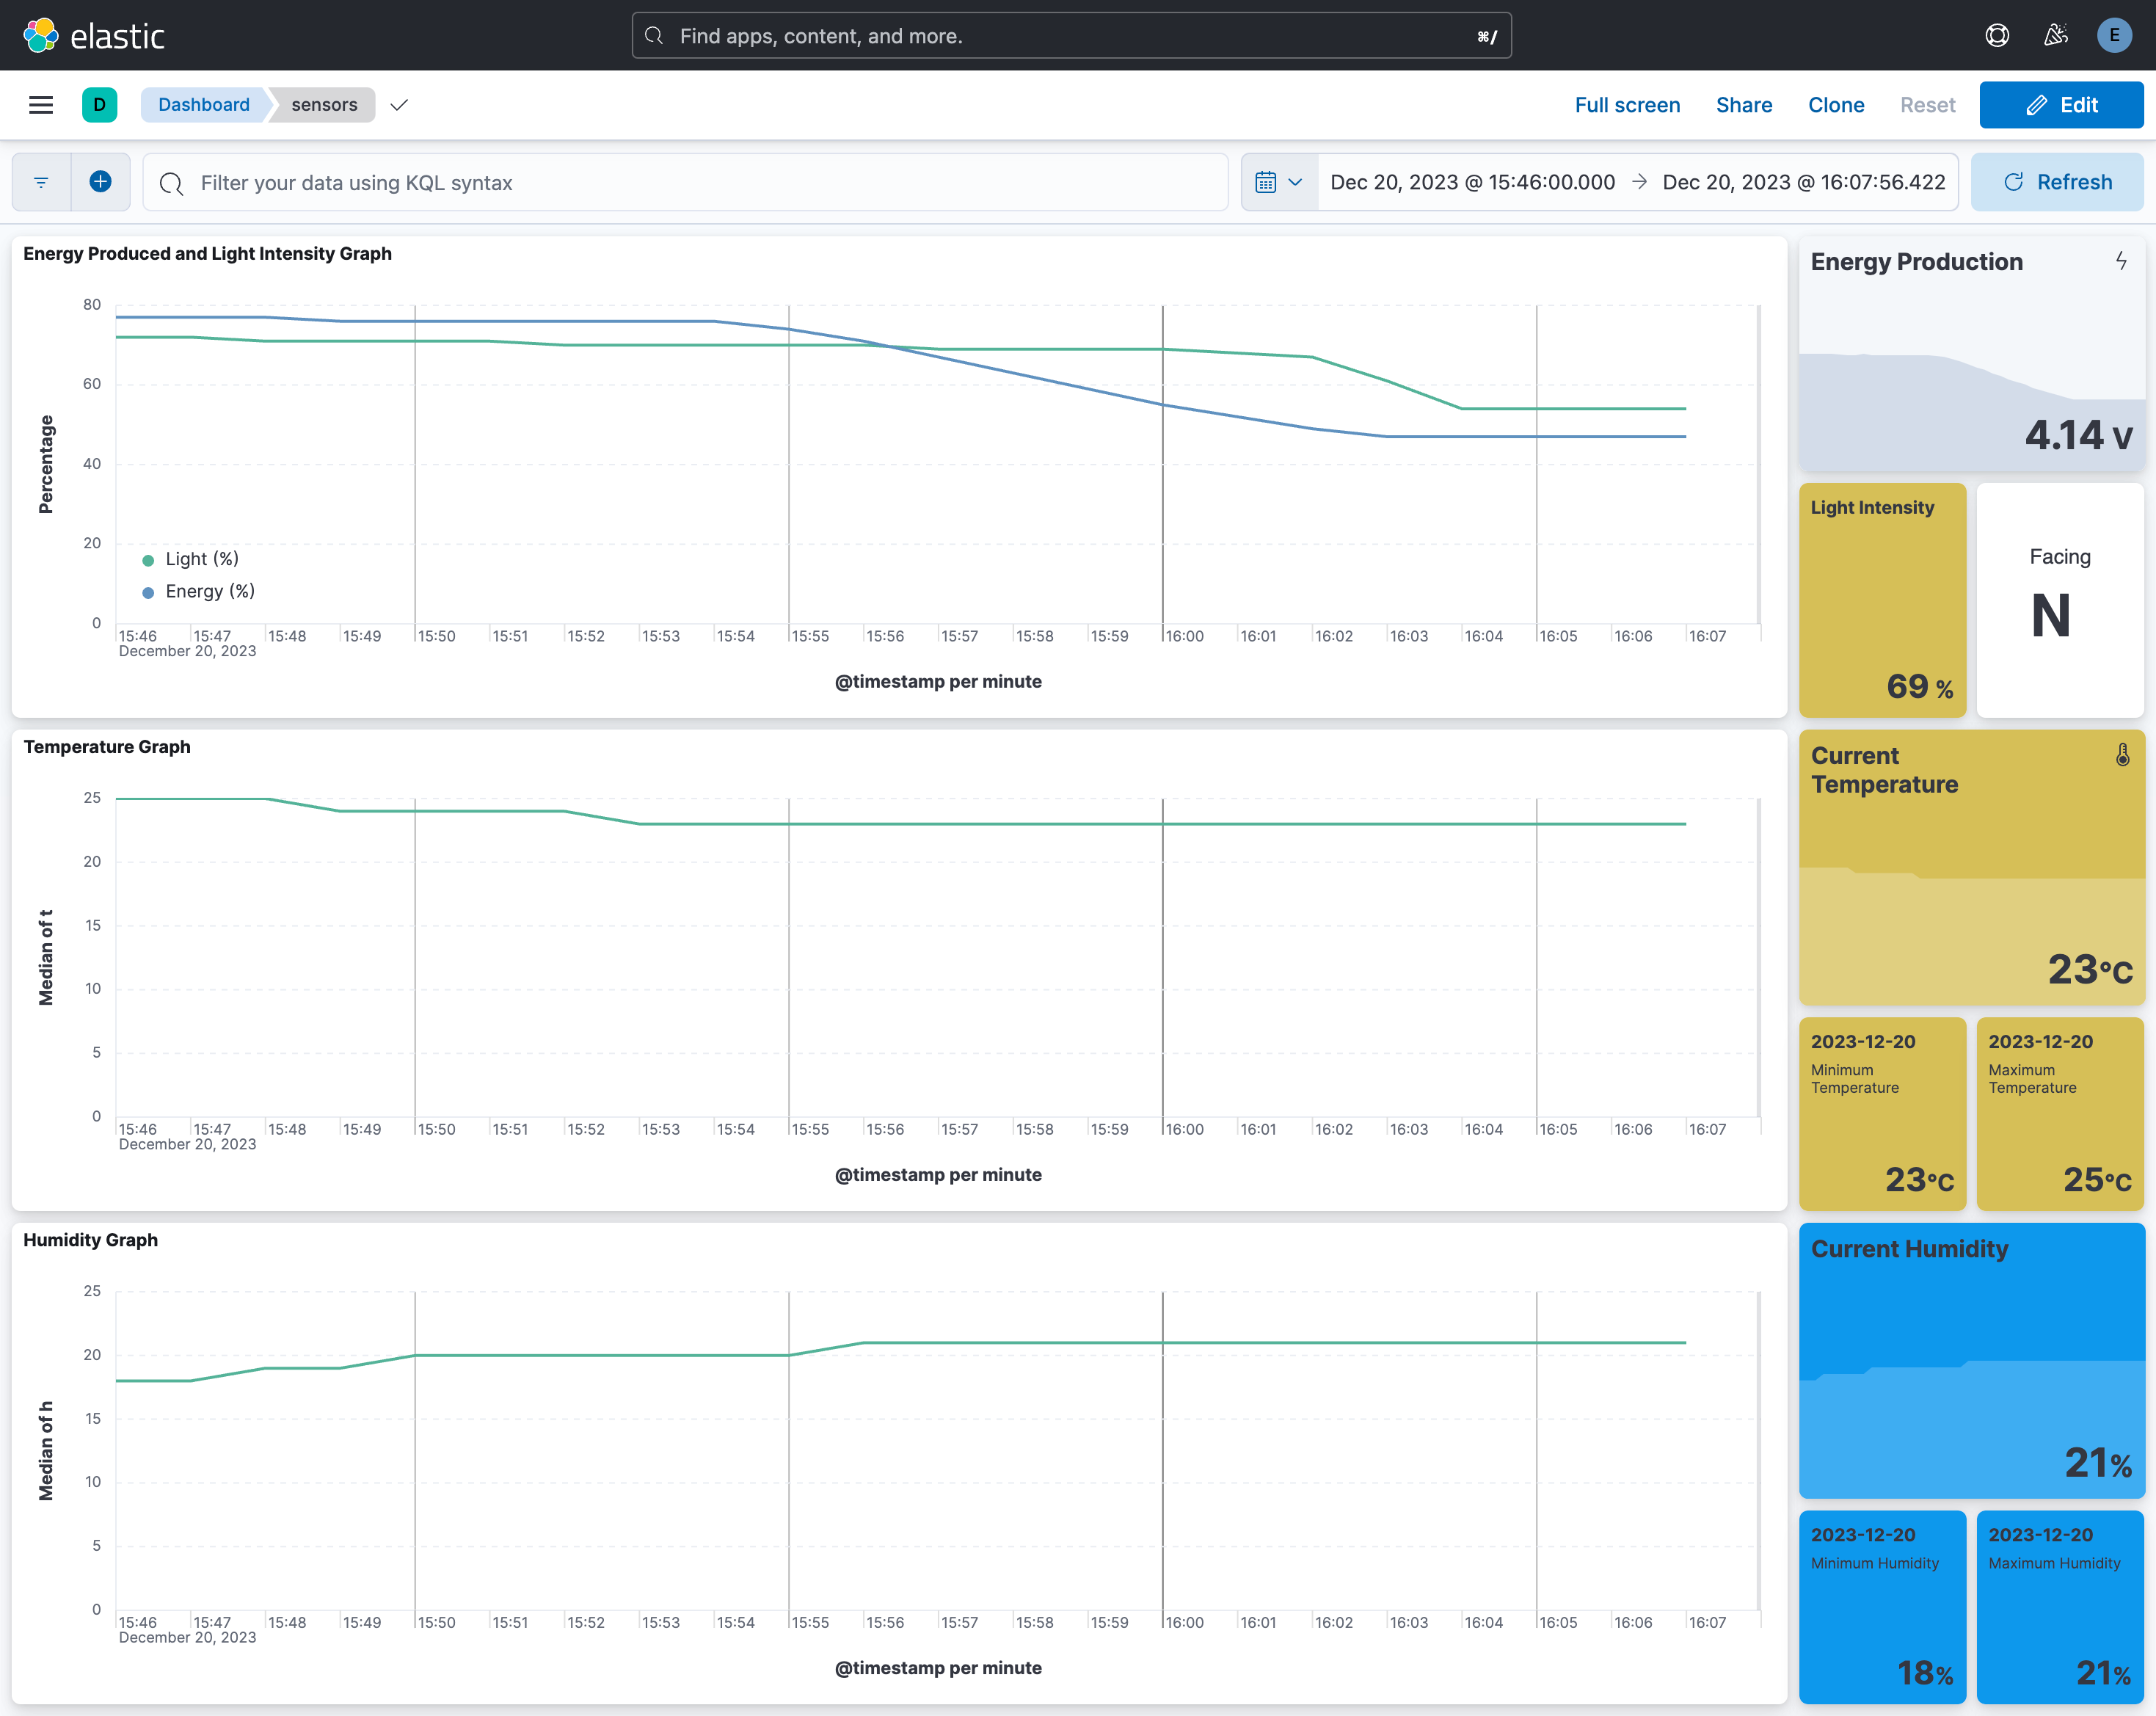
\includegraphics[width=\linewidth]{../assets/png/kibana-dashboard.png}
    \caption{The IoT Solar Station Kibana Dashboard.}
    \label{fig:kib}
\end{figure}\


\addcontentsline{toc}{section}{References}
\bibliographystyle{IEEEtran}
\bibliography{bibliography/bibliography}

\end{document}
